\documentclass[12pt,english]{scrartcl}

\usepackage{amsmath,amssymb}
%\usepackage[amssymb]{SIunits}
\usepackage{babel}
\usepackage[latin1]{inputenc}
\usepackage{graphicx}
\usepackage{color}


\begin{document}

\begin{center}
\textbf{\begin{LARGE}KOGW-PM-KNP:\\ \vspace{3mm} Tutorial 7 - Eye movement analysis
\end{LARGE}}
\end{center}

\noindent In this exercise you will be working through Python code (step\_by\_step\_quant.py) provided to you. The bulk of the code is broken up into auxiliary (aux\_funcs.py) and quantification (quant\_funcs.py) functions, stored in their respective scripts. You may views these functions for additional understanding but the focus here is on the concepts discussed in the following questions. \\

\begin{figure}[htbp]
\begin{center}
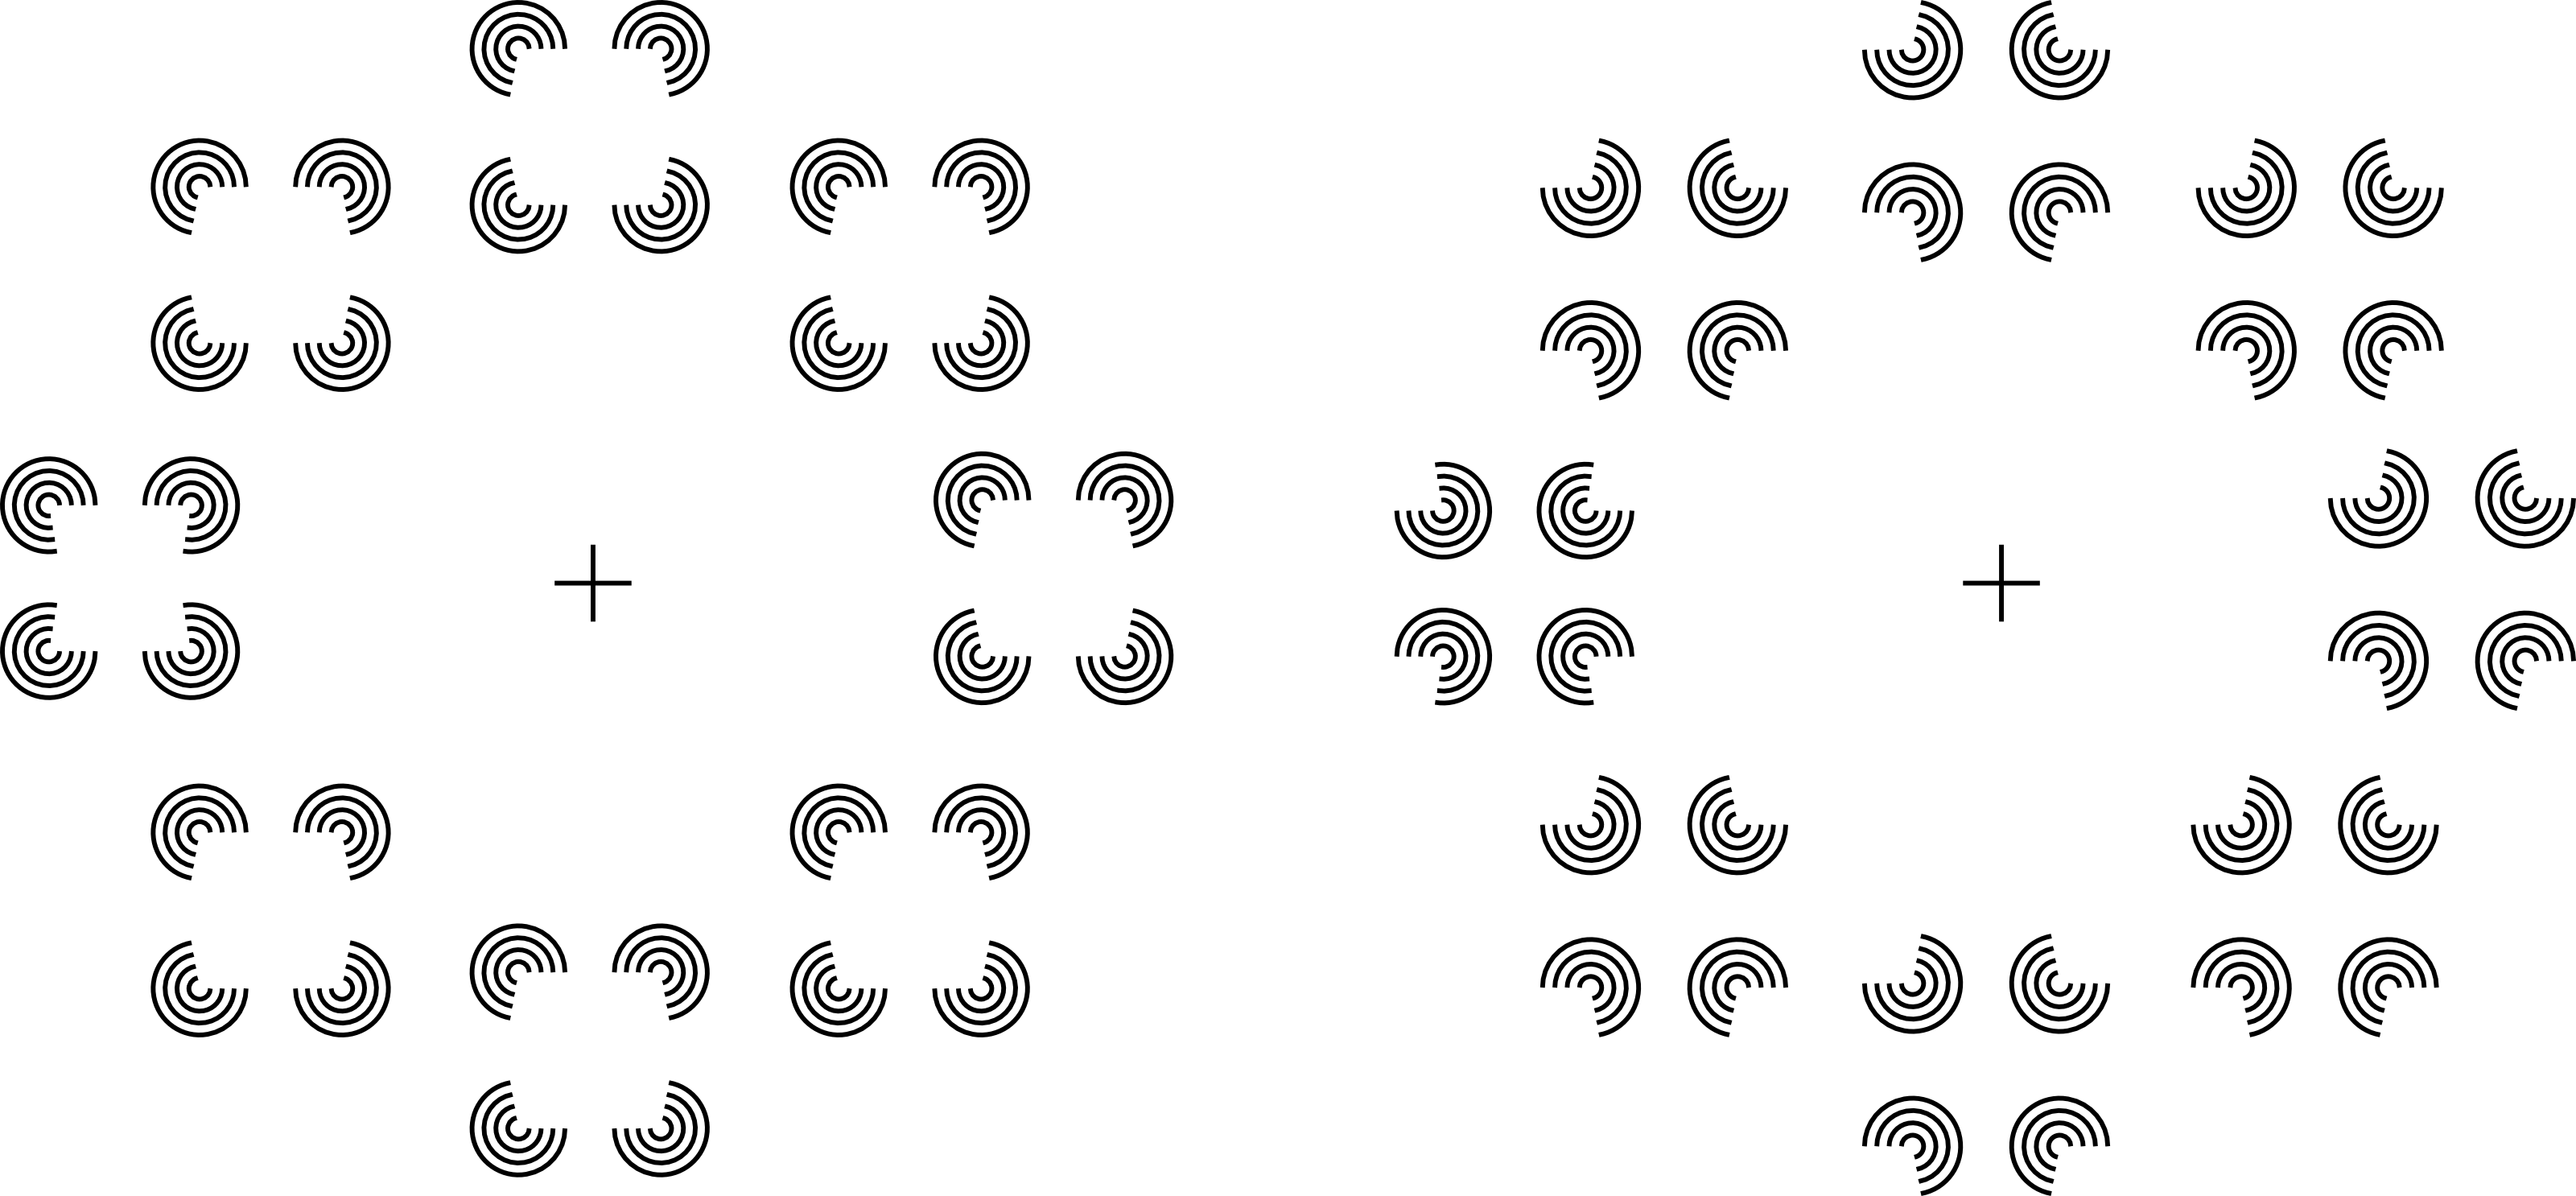
\includegraphics[width = 0.7\textwidth]{varin_search_display.png}
\end{center}
\caption{Search display in aligned and misaligned trials.The target is present at a 9 o'clock position in both types of display.
\label{fig:search}}
\end{figure}

\noindent To better understand the data here comes a short description of the experiment. Eye movements of the observers were measured while they searched for the odd-one-out in displays like the ones shown in Figure \ref{fig:search}. Eye positions (x,y on the screen) are registered every few milliseconds. An analysis of the eye movements provides insights of the processes involved in visual search in particular where and for how long observers fixate. \\

\noindent Before you start with the analysis remember to set the current directory to the folder containing the code and data (with "cd /location")


\begin{enumerate}
\item Lets first get familiar with the data. Look through the code and find where 'bdata', 'edata' are imported. Run the code up to 'edata'. Type 'bdata.keys()'. this displays the variable names of all the variables that we collected. Here comes an explanation what the different names stand for:
'rt' - reaction time, 'search' - target present or absent (1, 0), 'nitems' - number of items in the display (4, 8, 12), 'trl' - trial number, 'button' - button pressed by the observer, 'tpos\_x' - target position in x-direction, 'rot\_offset' - random offset of the items relative to 12 o'clock position on a circle, 'blk' - block number, 'tpos\_y' - target position in y-direction, 'target' - type of figure (1 - aligned, 0 - misaligned).

\item Do the first plotting. The figure shows an aligned and a misaligned configuration and a scan path for a trial with misaligned elements (target==0) and nitems==4. Do the more complex plot. It shows scan paths for different number of items (4,8 and 12 in rows) and three different example trials (columns).\\ 

Change the variables target from 0 to 1, and search from 0 to 1 and observe the differences in the scan paths. Note that you want to end up with 4 different plots (target: aligned, misaligned x search: present, absent). Make sure that you modify the subset of the data after you change the target.\\

%  \color{blue}
%  When the non identical inducer is present, the condition ends. This is when the participant would indicate with a button that they have noticed it. 
 
 \color{black}
 \item Having seen the raw data, we want to extract fixation points from the scan path. Considering your answer to the previous question, why might we be interested in the fixation points? One method to extract fixations from raw data  is based on a velocity threshold. Can you think of a way how this might work? \\
 
%  \color{blue}
%  \begin{itemize}
% item Fixations are eye movements below a certain thresholds, saccades are eye movements above the thresholds.  
%   \item Then we may be able to deduce what parts of the stimuli are used by the participants to discriminate between identical and non-identical inducers \\
%  
%   \item Velocity = distance / time . Therefore we can calculate the velocity by measuring the distance between subsequent points along the tracking path. \\
%  
%  \end{itemize}

 \color{black}
 \item The following code implements a velocity-based extraction of fixations. Follow the code through. Plot the intermediate results at various computation  steps from raw data to fixation points. Try to understand the different plots. The essential point is that below a certain velocity value, data points are defined as fixations, above the threshold they are defined as saccades. See what happens when you change the velocity threshold value to 20ms and 200ms.\\
 
%  \color{blue}
%  A lower threshold results in more fixation points. A higher threshold averages across these fixations. \\
 
 \color{black}
 \item Run the code for dispersion based quantification and read through its pseudo-code description. Note the difference in quality between this method and the previous. Try toying with the parameters for the duration threshold and minimum fixation threshold. What do you notice? 
%  \color{blue}
%  Dispersion correctly isolated more fixation points. \\
%  
%  The dispersion based method's parameters require more careful parameter setting. Changing them too much causes incorrect fixation detection. Note however, once stable detection parameters are found this method is much more robust. There are often such trade-offs between quantification methods.
%   

 \end{enumerate}
 \color{black}

\end{document}